\documentclass[a4paper]{article}
\usepackage[utf8]{inputenc}
\usepackage{fancyhdr}
\usepackage{vmargin}
\usepackage{listings}

%nicer tables
\usepackage{booktabs}

\usepackage{graphicx}

\usepackage{float}

\usepackage{color}
\usepackage{url}
\usepackage{hyperref}

\usepackage{enumerate}

\usepackage[backend=biber]{biblatex}

\usepackage{multicol}
\setlength{\columnsep}{1cm}
\setlength{\headheight}{36pt}

\definecolor{bluekeywords}{rgb}{0.13,0.13,1}
\definecolor{greencomments}{rgb}{0,0.5,0}
\definecolor{redstrings}{rgb}{0.9,0,0}



%
\usepackage{amsmath, amsthm, amssymb}
\usepackage[ngerman, english]{babel}
\usepackage{marvosym}
\usepackage{graphics}
\usepackage{extarrows}
\usepackage{forloop}
\usepackage{mathtools}

\usepackage[]{algorithm2e}

\usepackage{hyperref}% http://ctan.org/pkg/hyperref
\usepackage{cleveref}% http://ctan.org/pkg/cleveref
\usepackage{lipsum}% http://ctan.org/pkg/lipsum
\newtheorem{definition}{Definition}
\newtheorem{theorem}{Theorem}
\newtheorem{lemma}{Lemma}
\newtheorem{preliminary}{Preliminary}
\newtheorem{notation}{Notation}
\newtheorem{property}{Property}
\newtheorem{corollary}{Corollary}
\newtheorem{example}{Example}
\newtheorem{hypothesis}{Hypothesis}

\crefname{theorem}{Theorem}{Theorems}
\crefname{definition}{Definition}{Definitions}
\crefname{lemma}{Lemma}{Lemmas}
\crefname{preliminary}{Preliminary}{Preliminaries}
\crefname{notation}{Notation}{Notations}
\crefname{property}{Property}{Properties}
\crefname{corollary}{Corollary}{Corollaries}
\crefname{example}{Example}{Examples}
\crefname{hypothesis}{Hypothesis}{Hypotheses}

\newenvironment{beweis}{\begin{proof}[Beweis]}{\end{proof}}
%



\lstset{language=Python,
showspaces=false,
showtabs=false,
breaklines=true,
showstringspaces=false,
breakatwhitespace=true,
escapeinside={(*@}{@*)},
commentstyle=\color{greencomments},
keywordstyle=\color{bluekeywords}\bfseries,
stringstyle=\color{redstrings},
basicstyle=\ttfamily
}


\setlength{\parindent}{0pt}
\setlength{\parskip}{5pt}

\frenchspacing
\pagestyle{fancy}
\sloppy 

\markright{headline}

\addbibresource{references.bib}

\begin{document}

\lhead{\begin{tabular}{l}
\\
Neural Networks\\
Saarland University WiSe 2020/2021\\
\end{tabular}}

\rhead{\begin{tabular}{r}
Assignment 3\\
Simon Laurent Lebailly, 2549365\\%% <=== Also HERE if you have a team mateUpdate Name HERE !!! 
Christian Schmidt, 2537621
\end{tabular}}




\section*{Exercise 1: Linear Regression}
    \subsection*{1.1 Part a}
        \subsubsection*{a)}
            A unit change of $X_1$ can not always cause a $1000$ percent change in $Y$.
            Our equation is
            $$Y_i = 10 + 10 X_{i1} + 0.5 \log(X_{i2}) - 5 X_{i3}$$
            If we execute a $a$ unit change $X_1$, we receive
            $$Y'_i = 10 + 10 (X_{i1} + a) + 0.5 \log(X_{i2}) - 5 X_{i3}$$
            And further
            $$Y'_i = Y_i + 10a = Y_i + 10$$
            for $a=1$ and
            $$Y'_i = Y_i + 10a = Y_i - 10$$
            for $a=-1$.
            As example if we set $X_1 = X_2 = X_3 =1$ we receive $Y_i = 15$ and therefore $Y'_i = 15+10=25$ for $a=1$.
            So the one unit change of $X_1$ causes only a $167\%$ change of $Y$.
        
        \subsubsection*{b)}
            A unit change of $X_2$ can not always cause a $50$ percent change in $Y$.
            Our equation is
            $$Y_i = 10 + 10 X_{i1} + 0.5 \log(X_{i2}) - 5 X_{i3}$$
            If we execute a $a$ unit change $X_2$, we receive
            $$Y'_i = 10 + 10 X_{i1} + 0.5 \log(X_{i2} + a) - 5 X_{i3}$$
            And further
            $$Y'_i = 10 + 10 X_{i1} + 0.5 \log(X_{i2} + 1) - 5 X_{i3}$$
            for $a=1$ and
            $$Y'_i = 10 + 10 X_{i1} + 0.5 \log(X_{i2} - 1) - 5 X_{i3}$$
            for $a=-1$.
            As example if we set $X_1 = X_2 = X_3 =1$ we receive $Y_i = 15$ and therefore $Y'_i \approx 15 + 0,3466 = 15,3466$ for $a=1$.
            So the one unit change of $X_1$ causes only a $102,3\%$ change of $Y$.
        
        \subsubsection*{c)}
            A $100$ percent change of $X_3$ can not always cause a $50$ percent change in $Y$.
            Our equation is
            $$Y_i = 10 + 10 X_{i1} + 0.5 \log(X_{i2}) - 5 X_{i3}$$
            If we execute a $a$ unit change $X_1$, we receive
            $$Y'_i = 10 + 10 X_{i1} + 0.5 \log(X_{i2}) - a * 5 X_{i3}$$
            And further
            $$Y'_i = 10 + 10 X_{i1} + 0.5 \log(X_{i2}) - 2 * 5 X_{i3}$$
            for $a=2$ and
            $$Y'_i = 10 + 10 X_{i1} + 0.5 \log(X_{i2}) + 2 * 5 X_{i3}$$
            for $a=-2$.
            As example if we set $X_1 = X_2 = 1$, and $X_3 = 2$, we receive $Y_i = 10$ and therefore $Y'_i = 10 + 20 = 30$ for $a=-2$.
            So the $100$ percent change of $X_1$ causes a $300\%$ change of $Y$.

        \subsubsection*{d)}
            There is no correlation between depts and the future stock values.
            The future stock value can be higher to the actual stock value even if the depts were high.
        
        \subsubsection*{e)}
            $\beta_0$ is the start value of the company.
        
    \subsection*{1.2 Part b: Ridge Regression}
        to show: $w = \left({x^{(train)}}^T x^{(train)} + \lambda I \right)^{-1} {x^{(train)}}^T y^{(train)}$
        \begin{proof}
            $$J(w) = MSE_{train} + \lambda w^T w$$
            First we compute the derivative of $J$ with respect to $w$:
            \begin{align*}
                \nabla_w J(w) &= \nabla_w MSE_{train} + \nabla_w \lambda w^T w\\
                &= \nabla_w  \frac{1}{m} {\left\Vert \left( \hat{y}^{(train)} - y^{(train)} \right) \right\Vert}^2_2 + \nabla_w \lambda w^T w\\
                &= \nabla_w \frac{1}{m} {\left\Vert \left( w^T x^{(train)} - y^{(train)} \right) \right\Vert}^2_2 + \nabla_w \lambda w^T w\\
                &= \nabla_w \frac{1}{m} {\left\Vert \left( x^{(train)} w - y^{(train)} \right) \right\Vert}^2_2 + \nabla_w \lambda w^T w\\
                &= \nabla_w \frac{1}{m} \left( x^{(train)} w - y^{(train)} \right)^T \left( x^{(train)} w - y^{(train)} \right) + \nabla_w \lambda w^T w\\
                &= \nabla_w \frac{1}{m} \left( x^{(train)} w - y^{(train)} \right)^2 + \nabla_w \lambda w^2\\
                &= \frac{2}{m} {x^{(train)}}^T \left( x^{(train)} w - y^{(train)} \right) + 2 \lambda w
            \end{align*}
            Now we will find the corresponding extrema:
            \begin{align*}
                & & \frac{2}{m} {x^{(train)}}^T \left( x^{(train)} w - y^{(train)} \right) + 2 \lambda w &= 0\\
                &\Leftrightarrow &  \frac{2}{m} {x^{(train)}}^T \left( x^{(train)} w - y^{(train)} \right) + 2 \lambda w &= 0\\
                &\Leftrightarrow &  \frac{1}{m} {x^{(train)}}^T \left( x^{(train)} w - y^{(train)} \right) + \lambda w &= 0\\
                &\Leftrightarrow &  {x^{(train)}}^T \left( x^{(train)} w - y^{(train)} \right) + \lambda m w &= 0\\
                &\Leftrightarrow &  {x^{(train)}}^T x^{(train)} w - {x^{(train)}}^T y^{(train)} + \lambda m w &= 0\\
                &\Leftrightarrow &  \left( {x^{(train)}}^T x^{(train)} + \lambda m I \right) w &= {x^{(train)}}^T y^{(train)}\\
                &\Leftrightarrow &  w &= {\left( {x^{(train)}}^T x^{(train)} + \lambda m I \right)}^{-1} {x^{(train)}}^T y^{(train)}\\
            \end{align*}
        \end{proof}
    
    

\newpage
\section*{Exercise 2: Training Basics}
    \subsection*{2.1 Part a}
        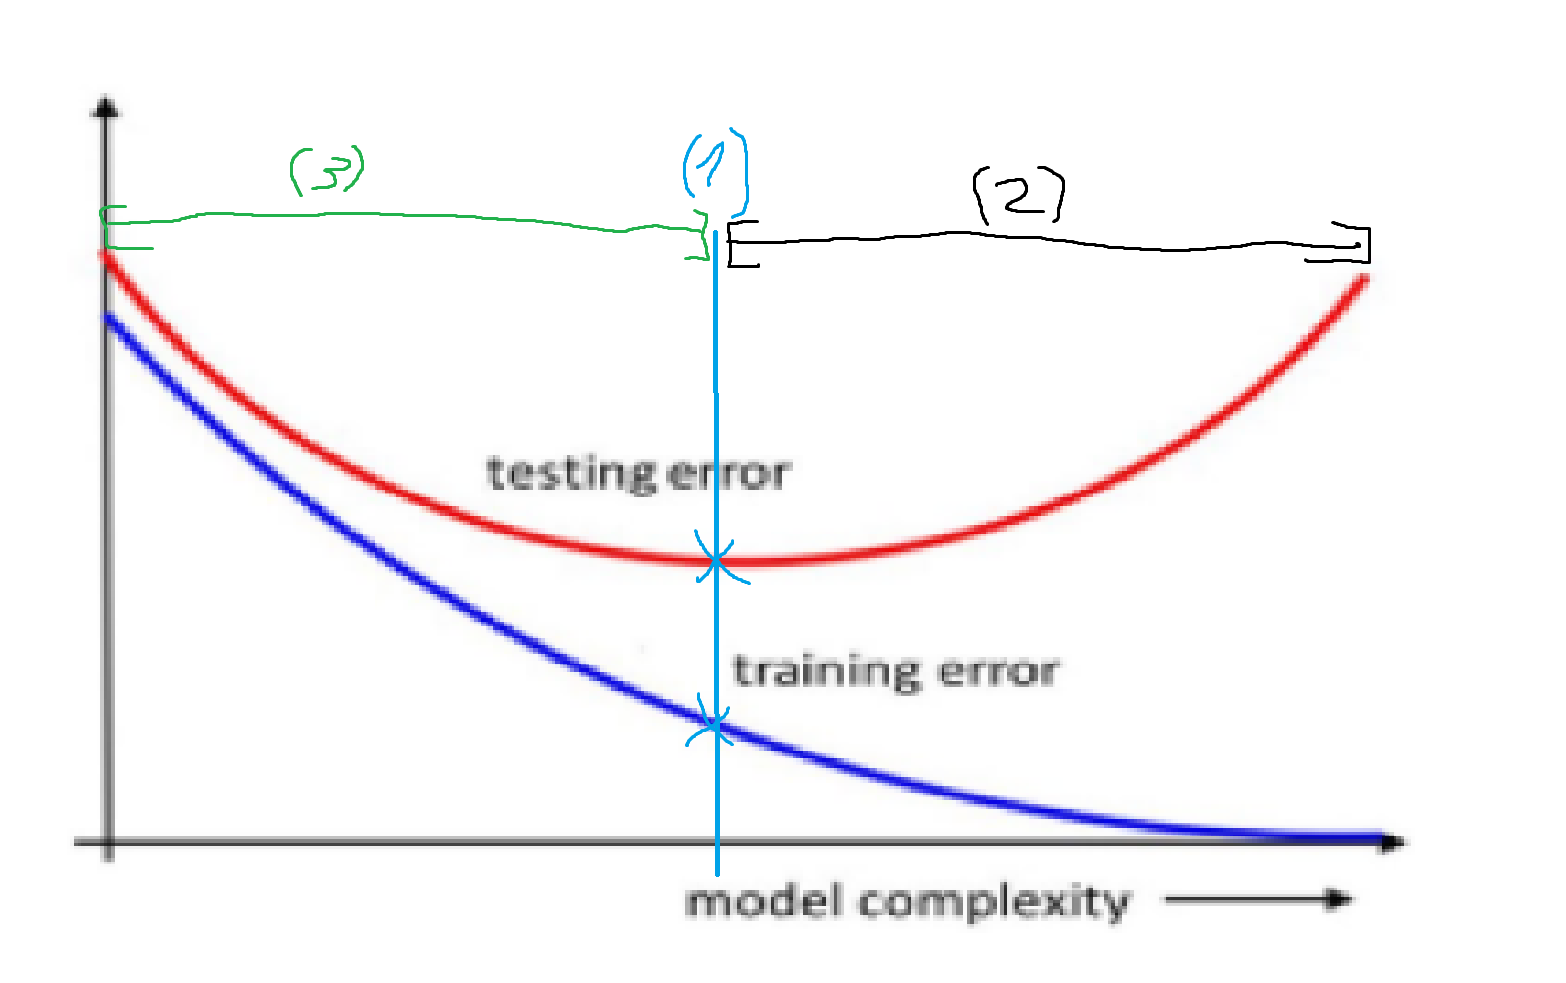
\includegraphics[width=0.6\linewidth]{2.1.png}
        \begin{itemize}
            \item The blue (1) marks the ideal point to operate the machine learning algorithm.
            \item The black (2) marks the range of the model complexity in which the machine learning algorithm overtrains/overfits.
            \item The green (3) marks the range of the model complexity in which the machine learning algorithm undertrains/underfits.
        \end{itemize}
        
        
    \subsection*{2.2 Part b}
        \subsubsection*{a)}
            If $\lambda$ increases, the slope of the model gets asymptotically close to zero.
            In other words, the larger $\lambda$ gets, the prediction becomes less and less sensitive to the weights.
            The idea is to increase the bias in order to decrease the variance, especially in overfitted models.
            
        \subsubsection*{b)}
        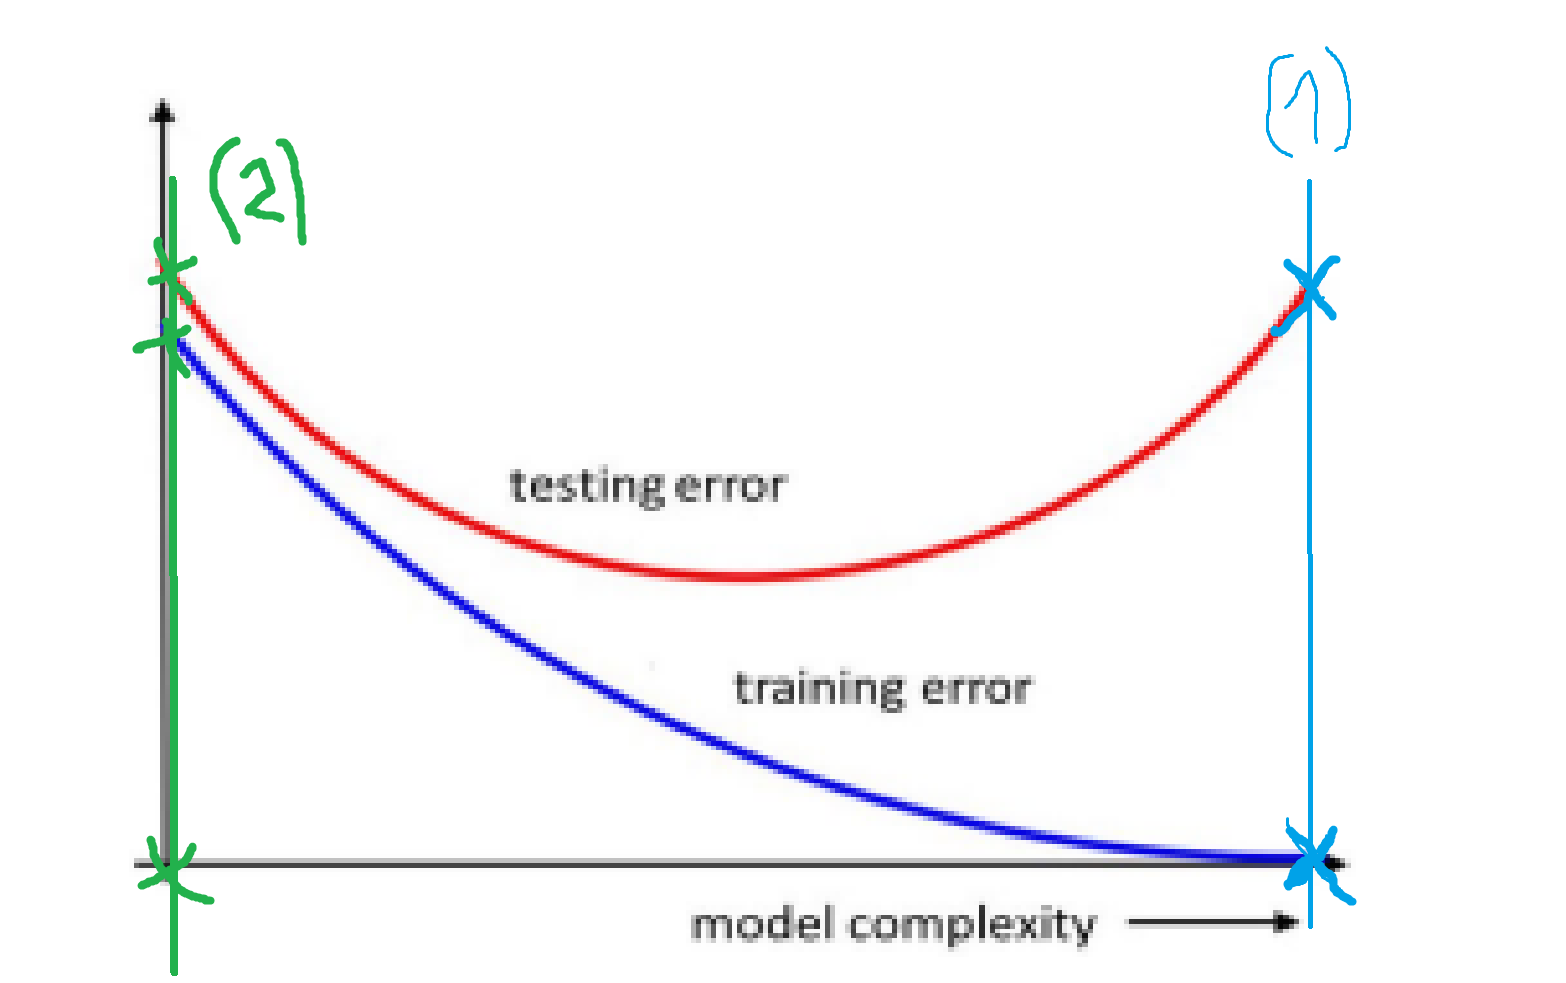
\includegraphics[width=0.6\linewidth]{2.2.png}
        \begin{itemize}
            \item The blue (1) marks the operating point if $\lambda=0$, because the system is overfitted. It has a low bias, but a high variance.
            \item The green (2) marks the operating point if $\lambda=\infty$, because the system "looks" untrained. It has a relatively high bias and variance. In this case, the linear function has no slope (horizontal).
        \end{itemize}
        
    \subsection*{2.3 Part c}
        


\newpage
\section*{Exercise 3: Maximum Likelihood}
    \subsection*{3.1 Part a}
        $$L(x_1,...,x_n;\lambda) = \prod\limits_{i=1}^n \frac{e^{-\lambda} \lambda^{x_i}}{x_i !}
        = \frac{e^{- n \lambda} \lambda^{x_1 + ... + x_n}}{x_1! \cdot ... \cdot x_n!}$$
        We estimate $\lambda$ by maximizing $\log L(x_1 ... x_n; \lambda)$:
        \begin{align*}
            \log L(x_1 ... x_n; \lambda) &= log \left( \frac{e^{- n \lambda} \lambda^{x_1 + ... + x_n}}{x_1! \cdot ... \cdot x_n!} \right)\\
            &= \log \left(e^{- n \lambda} \lambda^{x_1 + ... + x_n}\right) - \log \left(x_1! \cdot ... \cdot x_n!\right)\\
            &= \log \left(e^{- n \lambda}\right) + \log \left(\lambda^{x_1 + ... + x_n}\right) - \sum\limits_{i=1}^n \log \left(x_i !\right)\\
            &= \log \left(e^{- n \lambda}\right) + \log \left(\prod\limits_{i=1}^n \lambda^{x_i}\right) - \sum\limits_{i=1}^n \log \left(x_i !\right)\\
            &= \log \left(e^{- n \lambda}\right) + \sum\limits_{i=1}^n \log \left(\lambda^{x_i}\right) - \sum\limits_{i=1}^n \log \left(x_i !\right)\\
            &= -n \lambda + \log(\lambda) \sum\limits_{i=1}^n x_i - \sum\limits_{i=1}^n \log \left(x_i !\right)\ \ \ (I)
        \end{align*}
        The function is zero if all $x_1=...=X_n=0$.
        In the following we will consider the case that at least one $x_i \neq o$, $i \in \{1,...,n\}$.
        Now we compute the derivative of $\log L(x_1 ... x_n; \lambda)$ with respect to $\lambda$ to find a value that maximizes the function:
        $$\nabla_{\lambda} \log L(x_1,...,x_n;\lambda) = -n + \sum\limits_{i=1}^n \frac{x_i}{\lambda}$$
        To find the extrema:
        \begin{align*}
            & & \nabla_{\lambda} \log L(x_1,...,x_n;\lambda) &= 0\\
            &\Rightarrow &  -n + \sum\limits_{i=1}^n \frac{x_i}{\lambda} &= 0\\
            &\Leftrightarrow &  -n \lambda + \sum\limits_{i=1}^n x_i &= 0\\
            &\Leftrightarrow &  \lambda &= \sum\limits_{i=1}^n \frac{x_i}{n}\\
        \end{align*}
        Because of the nature of the function the only extrema $\lambda$ is a maximum!
        So we have find the maximum likelihood estimate of $\lambda$.
        
        
        
    \subsection*{3.2 Part b}



\newpage
\section*{Exercise 4: Logistic Regression}
    \subsection*{a)}
        In linear regression the outcome is continuous, so we have an infinite number of possible values.
        Whereas in logistic regression, the outcome has only a limited number of possible values.
        For example, if you want to specify the probability of events, it is not enough to use linear regression. 
        You have to make sure that you are always in the range of values between 0 and 1.
        However with linear regression we can not expect good categorical results.
        
    \subsection*{b)}
        Logistic regression is a supervised learning method. The data has to be well labeled!
        
    \subsection*{c)}
        No.
        
    \subsection*{d)}
        The coefficients of the logistic regression algorithm must be estimated from the training data. 
        The used training method for that is the maximum-likelihood estimation.
        
    \subsection*{e)}
        The output of logistic regression is categorial.
        Hence there is always a finite amount of possibilities, we know because of the decision boundaries, how high the probability for every category is and can compute the corresponding probability.

\newpage
\section*{Exercise 5}
    \subsection*{a)}
        Yes, the matrix $M$ is symmetric!
        \begin{itemize}
            \item A symmetric matrix has only real eigenvalues, and therefore the eigenvectors are also real.
            \item Asymmetric real matrix is a special case of a self-adjoint matrix with only real coefficients.
            \item The algebraic is equal to the geometric multiplicity of the eigenvalues.
            \item For a symmetric matrix mit normalized eigenvectors it holds
                $$M = S \cdot D \cdot S^{-1} = S \cdot D \cdot S^T$$
                with $S$ as ortgonal matrix with the normalized eigenvectors as columns. 
        \end{itemize}
        
        
    \subsection*{b)}
        A non-invertible matrix is called singular.\\
        However, per definition a matrix $M$ is invertible if, and only if, the determinant of $M$ is unequal zero!
        In other words, if $M$ is singular it holds that $det(M)=0$.\\
        It holds with the "rule of Sarrus":
        $$det(M) = \left| \begin{matrix} 1 & -1 & 0 \\ -1 & 2 & -1 \\ 0 & -1 & 1 \end{matrix} \right| = 2 - 1 - 1 = 0$$
        Hence the determinant of $M$ is zero, $M$ is singular!\\
        For the eigendecomposition it implies, that at least one eigenvalue is zero.
        
        
    \subsection*{c)}
            First we compute the \textbf{eigenvalues} with help of the "rule of Sarrus":
            \begin{align*}
                det(M) &= \left| \begin{matrix} (1-\lambda) & -1 & 0 \\ -1 & (2-\lambda) & -1 \\ 0 & -1 & (1-\lambda) \end{matrix} \right|\\ 
                &= (1 - \lambda)^2 (2 - \lambda) - 2 (1 - \lambda)\\
                &= (1 - 2\lambda + \lambda^2) (2 - \lambda) - 2 + 2\lambda\\
                &= 2 - \lambda - 4\lambda + 2\lambda^2 + 2\lambda^2 -\lambda^3 - 2 + 2\lambda\\
                &= -\lambda^3 + 4\lambda^2 - \lambda
            \end{align*}
            Now we can compute the eigenvalues:
                $$-\lambda^3 + 4\lambda^2 - \lambda = 0$$
                $$\Rightarrow \lambda_1 = 0 \text{ and } \lambda_2 = 3 \text{ and } \lambda_3 = 1$$
            
            In the next step we can compute the \textbf{eigenvectors}:
                \begin{enumerate}
                    \item For the frist eigenvalue $\lambda_1 = 0$:\\
                            $$M - \lambda_1 E = M$$
                        Solve the linear equation system $(M - \lambda_1E) \cdot v_1 = 0$:
                            $$\left ( \begin{array}{ccc} 1 & -1 & 0 \\ -1 & 2 & -1 \\ 0 & -1 & 1 \end{array} \right | \left. \begin{array}{c} 0 \\ 0 \\ 0 \end{array}\right)
                            \rightarrow \left ( \begin{array}{ccc} 1 & -1 & 0 \\ 0 & 1 & -1 \\ 0 & 0 & 0 \end{array} \right | \left. \begin{array}{c} 0 \\ 0 \\ 0 \end{array}\right)$$
                            $$\Rightarrow x_1 = x_2\ \ \  \wedge\ \ \  x_2 = x_3\ \ \  \wedge\ \ \  x_3 \text{ is arbitrarily selectable.}$$
                        So we have the general solution:
                            $$v_1 = \left( \begin{matrix} x_3 \\ x_3 \\ x_3 \end{matrix} \right) \text{, with } x_3 \in \mathbb{R}/\{0\}$$
                        Let $x_3 = 1$ and we become the eigenvector $v_1 = \left( \begin{matrix} 1 \\ 1 \\ 1 \end{matrix} \right)$
                        
                    \item For the second eigenvalue $\lambda_2 = 3$:\\
                            $$M - \lambda_2 E = M$$
                        Solve the linear equation system $(M - \lambda_2E) \cdot v_2 = 0$:
                            $$\left ( \begin{array}{ccc} -2 & -1 & 0 \\ -1 & -1 & -1 \\ 0 & -1 & -2 \end{array} \right | \left. \begin{array}{c} 0 \\ 0 \\ 0 \end{array}\right)
                            \rightarrow \left ( \begin{array}{ccc} 2 & 1 & 0 \\ 0 & 1 & 2 \\ 0 & 1 & 2 \end{array} \right | \left. \begin{array}{c} 0 \\ 0 \\ 0 \end{array}\right)
                            \rightarrow \left ( \begin{array}{ccc} 2 & 1 & 0 \\ 0 & 1 & 2 \\ 0 & 0 & 0 \end{array} \right | \left. \begin{array}{c} 0 \\ 0 \\ 0 \end{array}\right)$$
                            $$\Rightarrow x_1 = -\frac{1}{2} x_2\ \ \  \wedge\ \ \  x_2 = -2 x_3\ \ \  \wedge\ \ \  x_3 \text{ is arbitrarily selectable.}$$
                        So we have the general solution:
                            $$v_2 = \left( \begin{matrix} x_3 \\ -2 x_3 \\ x_3 \end{matrix} \right) \text{, with } x_3 \in \mathbb{R}/\{0\}$$
                        Let $x_3 = 1$ and we become the eigenvector $v_2 = \left( \begin{matrix} 1 \\ -2 \\ 1 \end{matrix} \right)$
                        
                    \item For the second eigenvalue $\lambda_3 = 1$:\\
                            $$M - \lambda_3 E = M$$
                        Solve the linear equation system $(M - \lambda_3E) \cdot v_3 = 0$:
                            $$\left ( \begin{array}{ccc} 0 & -1 & 0 \\ -1 & 1 & -1 \\ 0 & -1 & 0 \end{array} \right | \left. \begin{array}{c} 0 \\ 0 \\ 0 \end{array}\right)
                            \rightarrow \left ( \begin{array}{ccc} 1 & -1 & 1 \\ 0 & 1 & 0 \\ 0 & 1 & 0 \end{array} \right | \left. \begin{array}{c} 0 \\ 0 \\ 0 \end{array}\right)
                            \rightarrow \left ( \begin{array}{ccc} 1 & 0 & 1 \\ 0 & 1 & 0 \\ 0 & 0 & 0 \end{array} \right | \left. \begin{array}{c} 0 \\ 0 \\ 0 \end{array}\right)$$
                            $$\Rightarrow x_1 = -x_3\ \ \  \wedge\ \ \  x_2 = 0\ \ \  \wedge\ \ \  x_3 \text{ is arbitrarily selectable.}$$
                        So we have the general solution:
                            $$v_3 = \left( \begin{matrix} -x_3 \\ 0 \\ x_3 \end{matrix} \right) \text{, with } x_3 \in \mathbb{R}/\{0\}$$
                        Let $x_3 = 1$ and we become the eigenvector $v_3 = \left( \begin{matrix} -1 \\ 0 \\ 1 \end{matrix} \right)$
                \end{enumerate}
                Let $S = (v_1\ v_2\ v_3)$ be a matrix containing the eigenvectors of $M$ as columns.\\
                Hence the eigendecomposition of $M$ can be computed as follow:
                $$M = S \cdot D \cdot S^{-1} = (v_1\ v_2\ v_3) \cdot 
                \left( \begin{matrix} 0 & 0 & 0 \\ 0 & 3 & 0 \\ 0 & 0 & 1 \end{matrix} \right) \cdot (v_1\ v_2\ v_3)^{-1}$$
        
    

\end{document}
